%------------------------------------------------------------------------------
% SIMPLE TEMPLATE FOR P1 SCIENTIFIC JUSTIFICATION
% Use this template to generate the "scientific justification"
% for an ESO proposal for observing time, to be uploaded at
% https://www.eso.org/p1
%
% This LaTeX2e template is to be compiled with pdflatex.
% Import the resulting pdf file in the P1 interface.
% This file can be uploaded in a collaborative edition system like 
% OverLeaf.
%
% Do not tamper with the settings; changing the font size,
% margins, etc... may result in the proposal not being 
% considered.
% 

\documentclass[12pt]{article}
\usepackage[margin=3.0cm]{geometry}
\usepackage{authblk}
\title{Note on Quantum Information and Optimal Control}
\author[1]{Van Vincent Duong\thanks{vv2102@nyu.edu}}
\affil[1]{Department of Physics, New York Univesity, New York, NY, USA}
\usepackage{fancyhdr}
%\pagestyle{fancy}
%\rhead{Van Vincent Duong}
%\lhead{}
%\cfoot{}
%\rfoot{Page \thepage}
%\lfoot{\leftmark}
%\usepackage{palatino} % times font

\usepackage{listings}
\usepackage{comment}
\usepackage{float}

\setlength{\parskip}{0.5em}
\linespread{1}

\usepackage{amsmath}
\usepackage{amssymb}
\usepackage{graphicx}
\usepackage{subfigure}
\usepackage{subcaption}

\newcommand{\RE}{\mathrm{Re}}
\newcommand{\IM}{\mathrm{Im}}
\newcommand{\E}{\mathbb{E}}
\newcommand{\Tr}{\mathrm{Tr}}

%\renewcommand{\thesection}{}
%\renewcommand{\thesubsection}{}
%\renewcommand{\familydefault}{\sfdefault}
%\paperwidth 21cm
%\paperheight 29.7cm
%\textwidth 16.7cm
%\textheight25.7cm
%\oddsidemargin0cm \evensidemargin0cm
%\topmargin-2cm
%\parindent0cm
%\parskip0.3cm
%\usepackage{graphicx}
%\pagestyle{empty}

% Times new roman
%\usepackage{mathptmx}
% 2cm margins


\begin{document}


%------------------------------------------------------------------------------
\maketitle

\begin{abstract}
  
\end{abstract}

\newpage

\tableofcontents

\section{Quantum sensing}

In sensing, one tries to estimate an external field.  The prototypical quantum sensing example involves coupling a spin-1/2 state to an unknown magnetic field.  As the state evolves, one infers the magnetic field parameter that generates its dynamics.  The quantum state $\rho$ contains metrological information called the quantum Fisher information $F_Q$ -- and some states can increase the quantity $F_Q$.  This section connects quantum dynamics, information theory, and control.

In metrology, the goal is to maximise the quantum Fisher information $F_{Q}$ of the state concerning the external field.  For multiple parameter estimation $\vec{x}$, I define the quantum Fisher information matrix elements by
\begin{align}
    [F_Q]_{ab} = \frac{1}{2}\Tr\left[ \rho \{L_a, L_b\} \right],
\end{align}
where $L_a$ is the symmetric derivative satisfying $\partial_a \rho = \tfrac{1}{2}\{\rho, L_a \}$. For our purposes, the single parameter I want to estimate is $x$.  Note that the symmetric derivative admits an integral representation that can be useful later
\begin{align*}
    L_a = \int_{0}^{\infty} ds \, e^{-\frac{\rho s}{2}} [\partial_a \rho] e^{-\frac{\rho s}{2}}.
\end{align*}
By diagonalising the density matrix $\rho = U \Lambda U^\dagger$, I can write the quantum Fisher information $F_Q$ in a useful representation:
\begin{align}
    F_Q = 4 \sum_{ij} \frac{\lambda_i }{(\lambda_i + \lambda_j)^2}|\mathcal{D}_{ij}|^2,
\end{align}
where $\mathcal{D} = U^\dagger [\partial_x \rho] U$. In this form, the information is calculated with two objects: the density matrix $\rho$ and its derivative for the parameter $\partial_x \rho$. 

Let us shift our attention to the system's dynamics. I typically couple the quantum state $\rho$ to the external field using a Hamiltonian for quantum sensing purposes. The quantum state evolves according to the master equation $\partial_t \rho = \mathcal{L}[\rho]$, which accounts for noisy processes. The corresponding master equation reads
\begin{align}
    \partial_t \rho = & - i [H, \rho] + \sum_{i}\left( K_i \rho K_i^\dagger - \frac{1}{2}\{K_i^\dagger K_i, \rho \}\right),
\end{align}
where $K_i$ are the channel's Kraus operators. In general, I'll have access to a time-dependent control field, so the total Hamiltonian becomes
\begin{align}
H = H_0(\vec{x}) + \sum_{i=1}^{p} V_k(t) H_k.
\end{align}
The first term encodes the external field $x$ I want to sense, and the last is our control.  

In this note, I'll consider evolving a single spin-1/2 state in the presence of an external magnetic field and depolarising noise but with a control field:
\begin{align}
    H = & \frac{1}{2} \omega_0 \sigma_3 + \vec{V}(t) \cdot \vec{\sigma}\\
    K_i = & \sqrt{\gamma} \sigma_i.
\end{align}
The parameter $\omega_0$ is what I want to estimate, $\gamma>0$ is the dissipation rate, and $\vec{V}(t)$ is the control.

Performing the time-evolution of the density matrix $\rho(t)$ is non-trivial. One approach is discretising time and stepping in small intervals $\Delta t$ from the last state to the next using the master equation $\partial_t \rho = \mathcal{L}[\rho]$. Since the Lindblad operator $\mathcal{L}$ generates time translations, exponentiation allows us to perform the time evolutions. Defining the operator $K(t_i, t_j)$ as the propagator from one time ($t_j$) to a future time ($t_i$) allows us to write
\begin{align}
    \rho(t_n) = & K(t_n, t_0) \rho(t_0)\\
    = & K(t_n, t_{n-1}) \rho(t_{n-1})\\
    = & e^{\Delta t \mathcal{L}} \rho(t_{n-1}).
\end{align}
In this form, we are on our way to calculate the derivative $\partial_x \rho$ at each time step, a necessary ingredient for knowing the state's quantum Fisher information. The key idea is to calculate the derivative recursively. Turning the crank, I get
\begin{align}
    \partial_x \rho(t_n) = \left[ \partial_x e^{\Delta t \mathcal{L}} \right] \rho(t_{n-1}) + e^{\Delta t \mathcal{L}} \left[ \partial_x \rho(t_{n-1})\right].
\end{align}
Terms with $\rho(t_{n-1})$ are known from the last time step, while terms with $\mathcal{L}$ are calculated on the fly. 

Let's explicitly calculate the derivative $ \partial_a e^{\Delta t \mathcal{L}}$. A key integral representation of the derivative of the exponential map is key for any calculation. Namely, I have
\begin{align}
    \partial_a e^{O(x)} = \int_0^1 ds\, e^{s O(x)}\left[\partial_a O(x)\right]e^{(1-s) O(x)}.
\end{align}
Setting $\mathcal{L} \Delta t = O(x)$ and $\mathcal{L}_a \Delta t = \partial_a O(x)$ provides us with
\begin{align}
    \partial_a e^{\Delta t \mathcal{L}} = \Delta t \int_0^1 ds\, e^{s \mathcal{L} \Delta t}\left[\mathcal{L}_a\right]e^{(1-s) \mathcal{L} \Delta t}.
\end{align}
The integral is evaluated by diagonalising the Lindbladian $\mathcal{L} = V D V^\dagger$:
\begin{align}
    \partial_a e^{\Delta t \mathcal{L}} = & V A V^\dagger\\
   [A]_{ij} = & \frac{e^{\Delta t d_i} - e^{\Delta t d_j}}{d_i - d_j}\left[V^\dagger \mathcal{L}_a V\right]_{ij}.
\end{align}
The operator $\mathcal{L}_a$ is typically the dynamics generated by the conjugate operator $H_a$ to the field $x_a$. That is,
\begin{align}
    \mathcal{L}_a \rho = - i [H_a, \rho].
\end{align}
All these intermediate calculations allow for evaluating the derivative $\partial_a e^{\Delta t \mathcal{L}}$. 

In this section, I described the quantum Fisher information matrix $F_Q$. I also reviewed the dynamics of dissipative systems using the Lindblad master equation. Finally, I showed how to evaluate the quantum Fisher information with dynamics.

\subsection{Example (analytical): spin-1/2 particle with Pauli noise}

In this example, I analyse the quantum information of a spin-1/2 when it undergoes noisy dynamics.  Consider an arbitrary quantum state initialised at $\rho$ with the corresponding Lindblad equation
\begin{align}
    \partial_t \rho = & - i [H, \rho] + \sum_{i=1}^{3}\left( K_i \rho K_i^\dagger - \frac{1}{2}\{K_i^\dagger K_i, \rho \}\right),\\
    H = & \frac{1}{2}\omega \sigma_3,\\
    K_i = & \sqrt{\gamma} \sigma_i.
\end{align}
The time evolution of the state resembles that of a damped oscillator:
\begin{align}
    \rho(t) = &
    \begin{pmatrix}
    \frac{1}{2} + c_1 e^{- 4 \gamma t} & c_2 e^{- (4 \gamma + i \omega) t}\\
    c_2^* e^{- (4 \gamma - i \omega) t} & \frac{1}{2} - c_1 e^{- 4 \gamma t}
\end{pmatrix},
\end{align}
where the initial conditions fix $c_1, c_2$. A straightforward calculation shows the purity of the state decays exponentially
\begin{align}
    \Tr [\rho^2] = & 2\left(c_1{}^2+|c_2|^2\right) e^{-8 \gamma  t}+\frac{1}{2}.
\end{align}

I calculate the state's quantum Fisher information $F_Q$. The information with respect to $\omega$ is 
\begin{align}
    F_{Q} = 4 |c_2|^2 t^2 e^{-8 \gamma  t}.
\end{align}
There are competing effects.  In the early times, $F_Q$ grows quadratically but decays exponentially in the late times.  The maximum amount of information in the system is $|c_2|^2 e^{4}/\gamma^2$, which is attained at time $t=1/(4\gamma)$. Moreover, note the importance of the cross term $c_2$.  If it were not present, the state would contain zero information.  The inflection points are located at $t_{\pm} = (2 \pm \sqrt{2})/(8 \gamma)$. 

I also have information about the system's dissipation rate, $\gamma$.  The quantum Fisher information for $\gamma$ is
\begin{align}
    F_{Q} = & \frac{16 \left(c_1^2+|c_2|^2\right) t^2 }{ e^{8 \gamma t}-4(c_1^2+|c_2|^2)}\\
    = & 2t^2 \left(\frac{1}{\Tr[\rho^2]} - 2 \right).
\end{align}
and is approximately maximised at $t =(4(c_1^2 + |c_2|^2) - 1)/(12 \gamma)$.

\subsection{Example (numerics): spin-1/2 particle with Pauli noise}

In this example, I examine the same system with numerical techniques. My results serve to validate the matrix formulas I derived and their stability.

The dynamics are represented on the Bloch sphere and coincide with the theory.
\begin{figure}[ht]
    \centering
    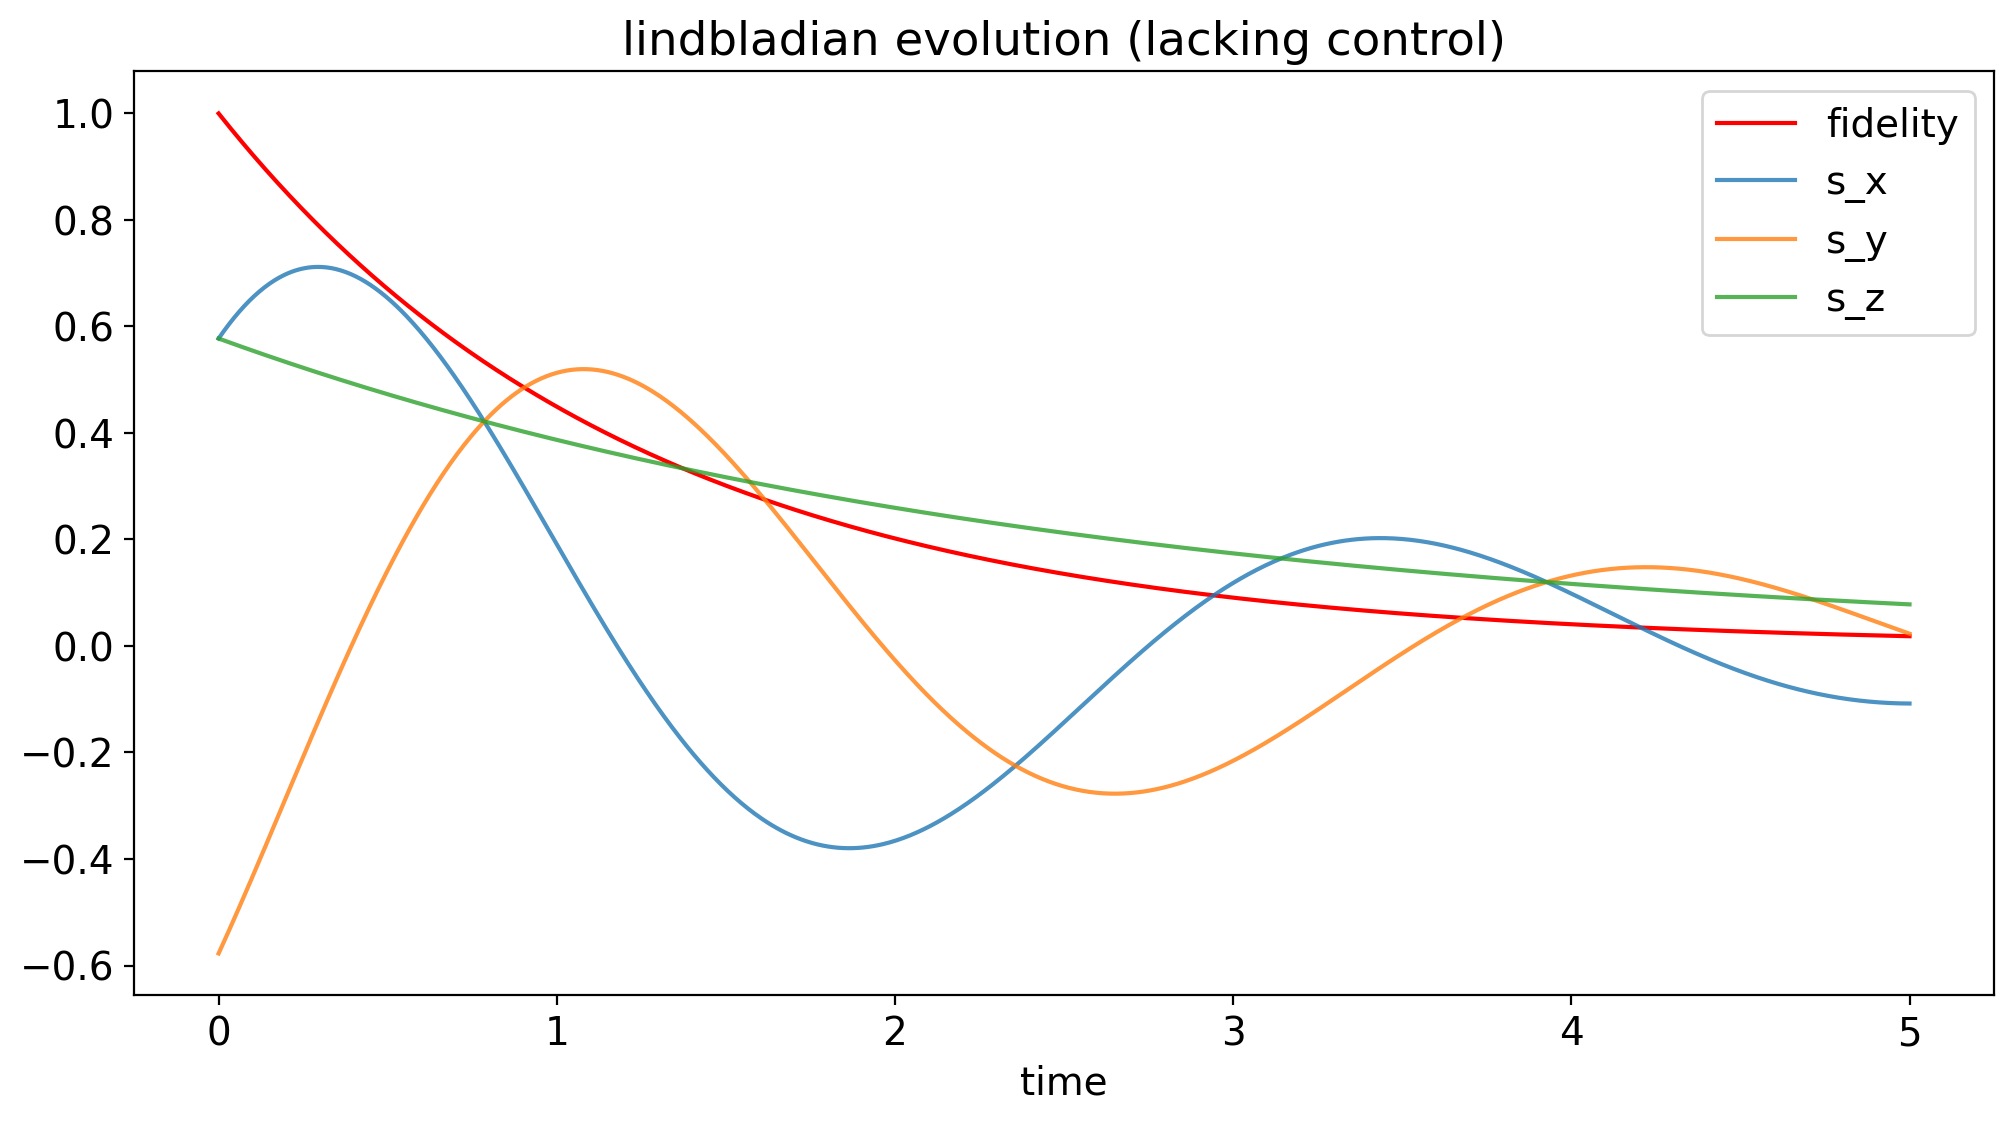
\includegraphics[width=12cm]{bloch_no_control.png}
    \caption{Bloch sphere dynamics and fidelity.}
    \label{fig: bloch_no_control}
    \centering
\end{figure}

I calculate the state's quantum Fisher information $F_Q$ for $\omega$. My numerical technique coincides with the theory.
\begin{figure}[ht]
    \centering
    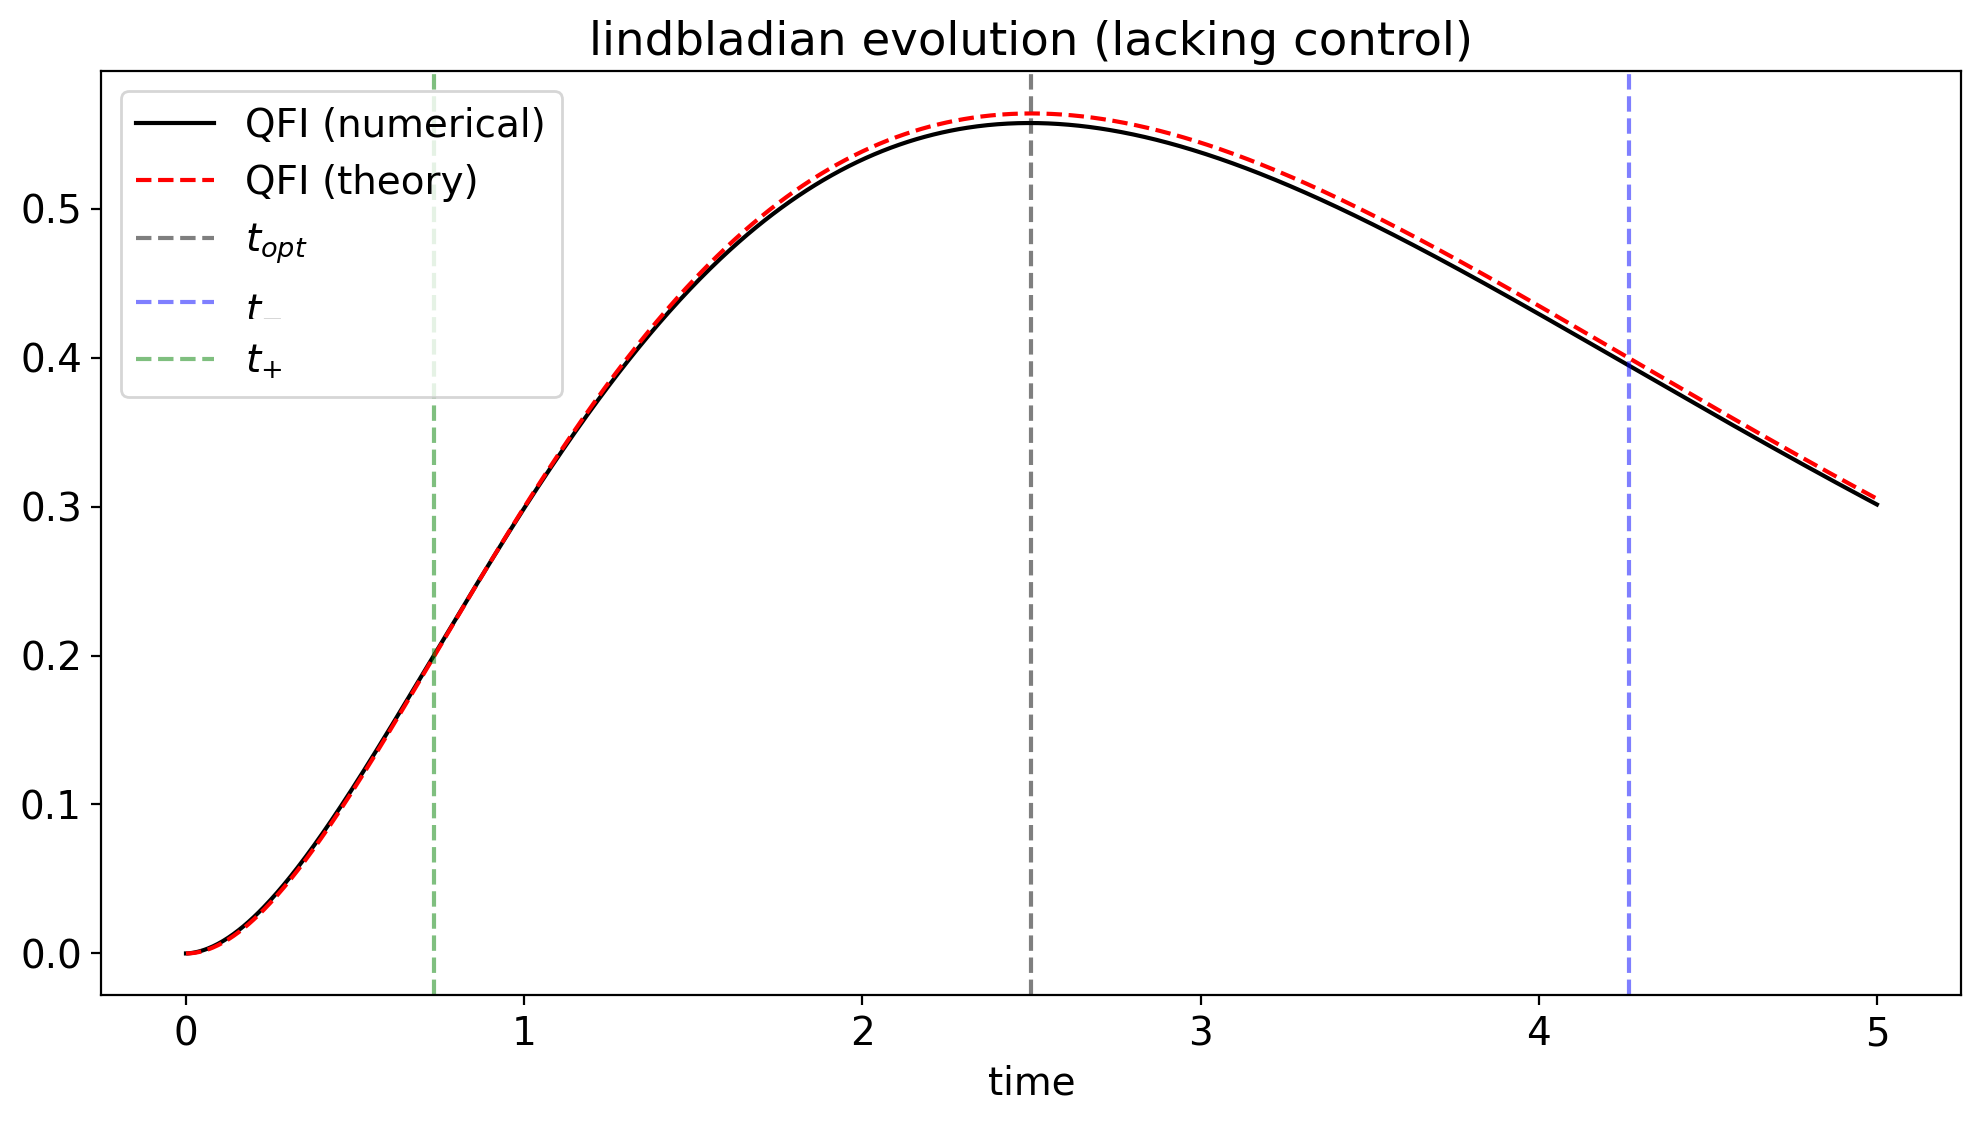
\includegraphics[width=12cm]{info_no_control.png}
    \caption{Quantum Fisher information with respect to $\omega$.}
    \label{fig: info_no_control}
    \centering
\end{figure}

\subsection{Example (numerics): controlling a spin-1/2 particle with Pauli noise}

I examine the same system with a control field $\vec{V}(t)$ in this example. Solving the time-dependent master equation is usually impossible so that I will use my numerical technique. The idea of a control field to improve a reward function is old. It has striking similarities to the concept of dynamical decoupling. 

The first control is
\begin{align}
    \vec{V}(t) = 0.5 (\cos(5 t), \cos(0.1 t), 0),
\end{align}
which I found via trial and error. Its dynamics are solved and shown in \ref{fig: bloch_yes_control}.
\begin{figure}[ht]
    \centering
    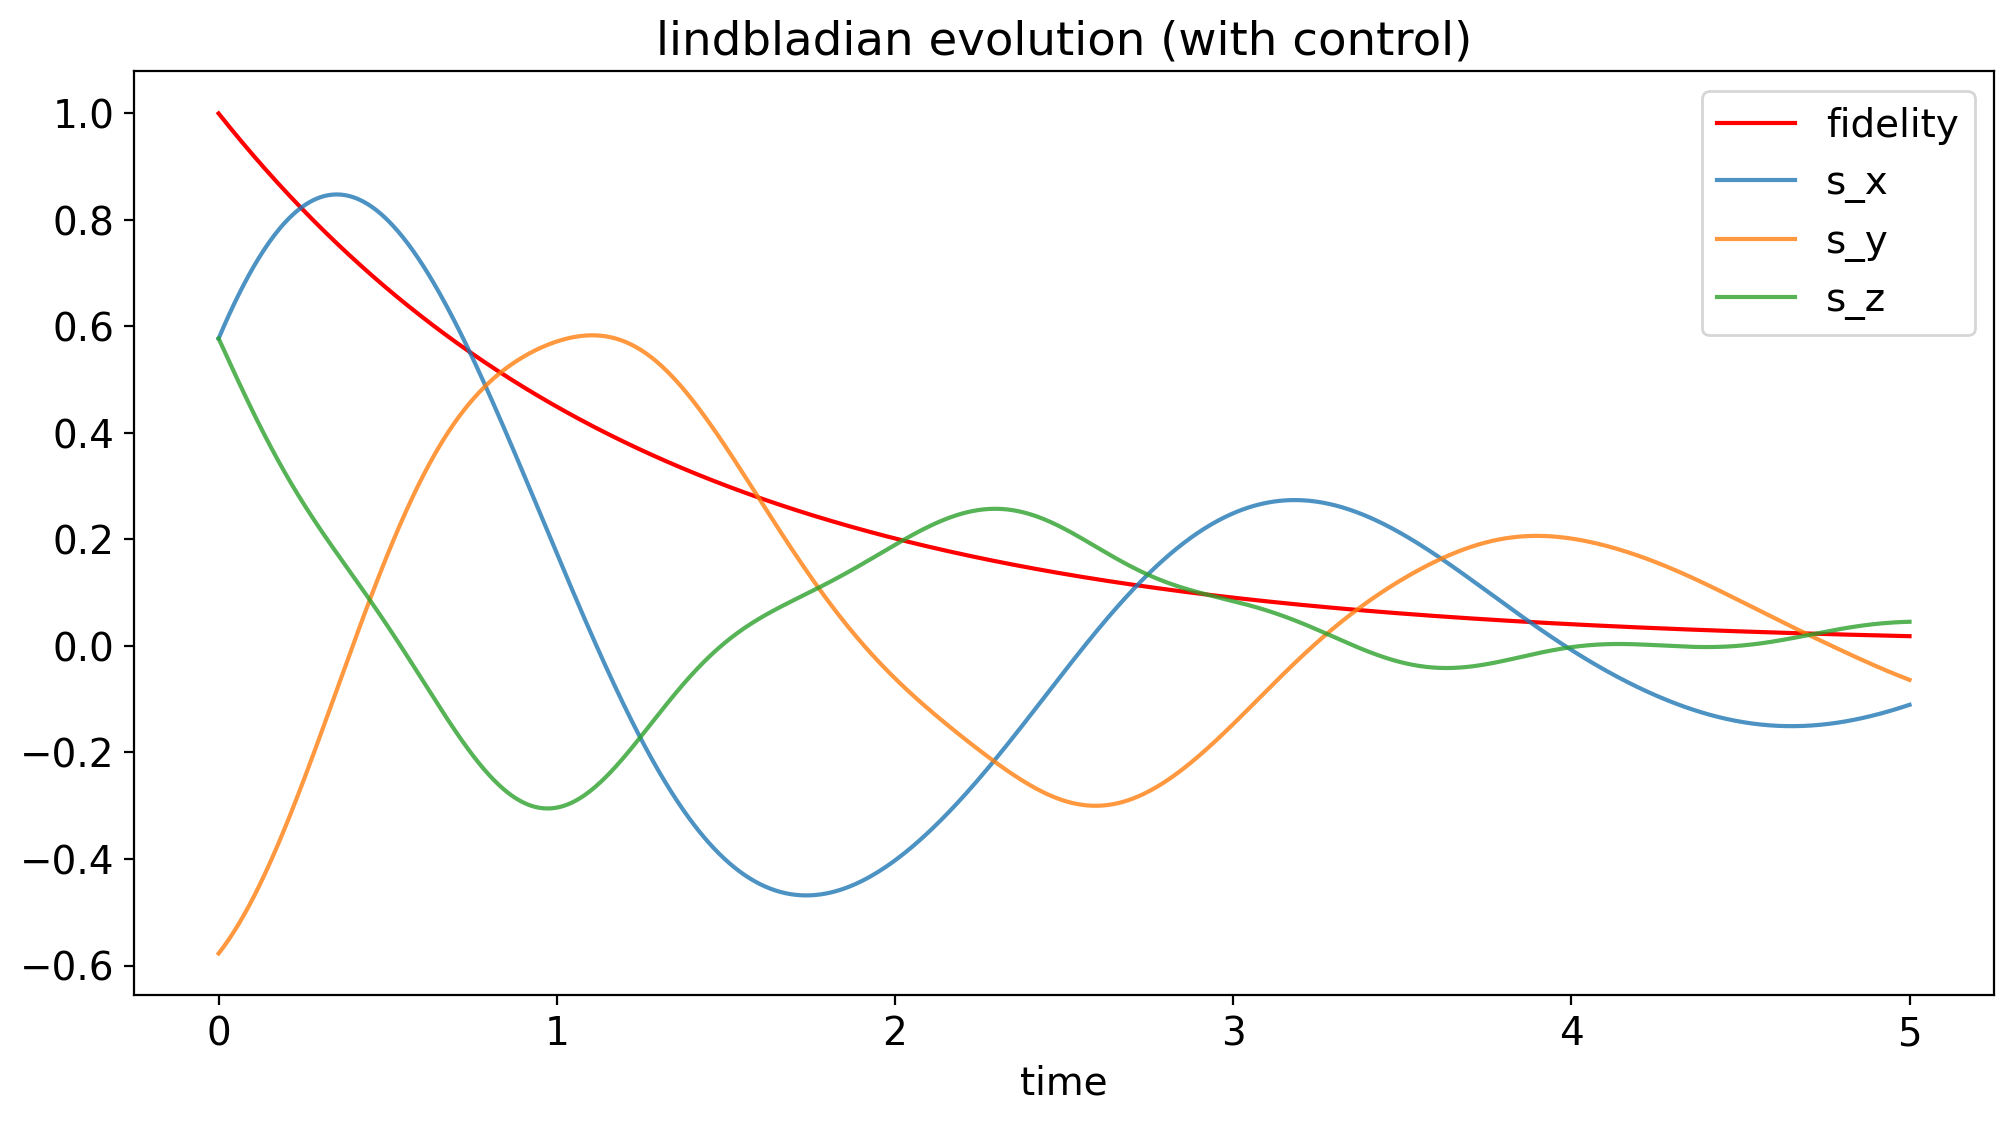
\includegraphics[width=12cm]{bloch_yes_control.png}
    \caption{Bloch sphere dynamics and fidelity.}
    \label{fig: bloch_yes_control}
    \centering
\end{figure}
I calculate the state's quantum Fisher information $F_Q$ for $\omega$. The control $\vec{V}(t)$ was chosen to improve the $F_Q$. (I tried many other controls, but most reduced the quantum Fisher information.) The improvement is shown in \ref{fig: info_yes_control}.
\begin{figure}[ht]
    \centering
    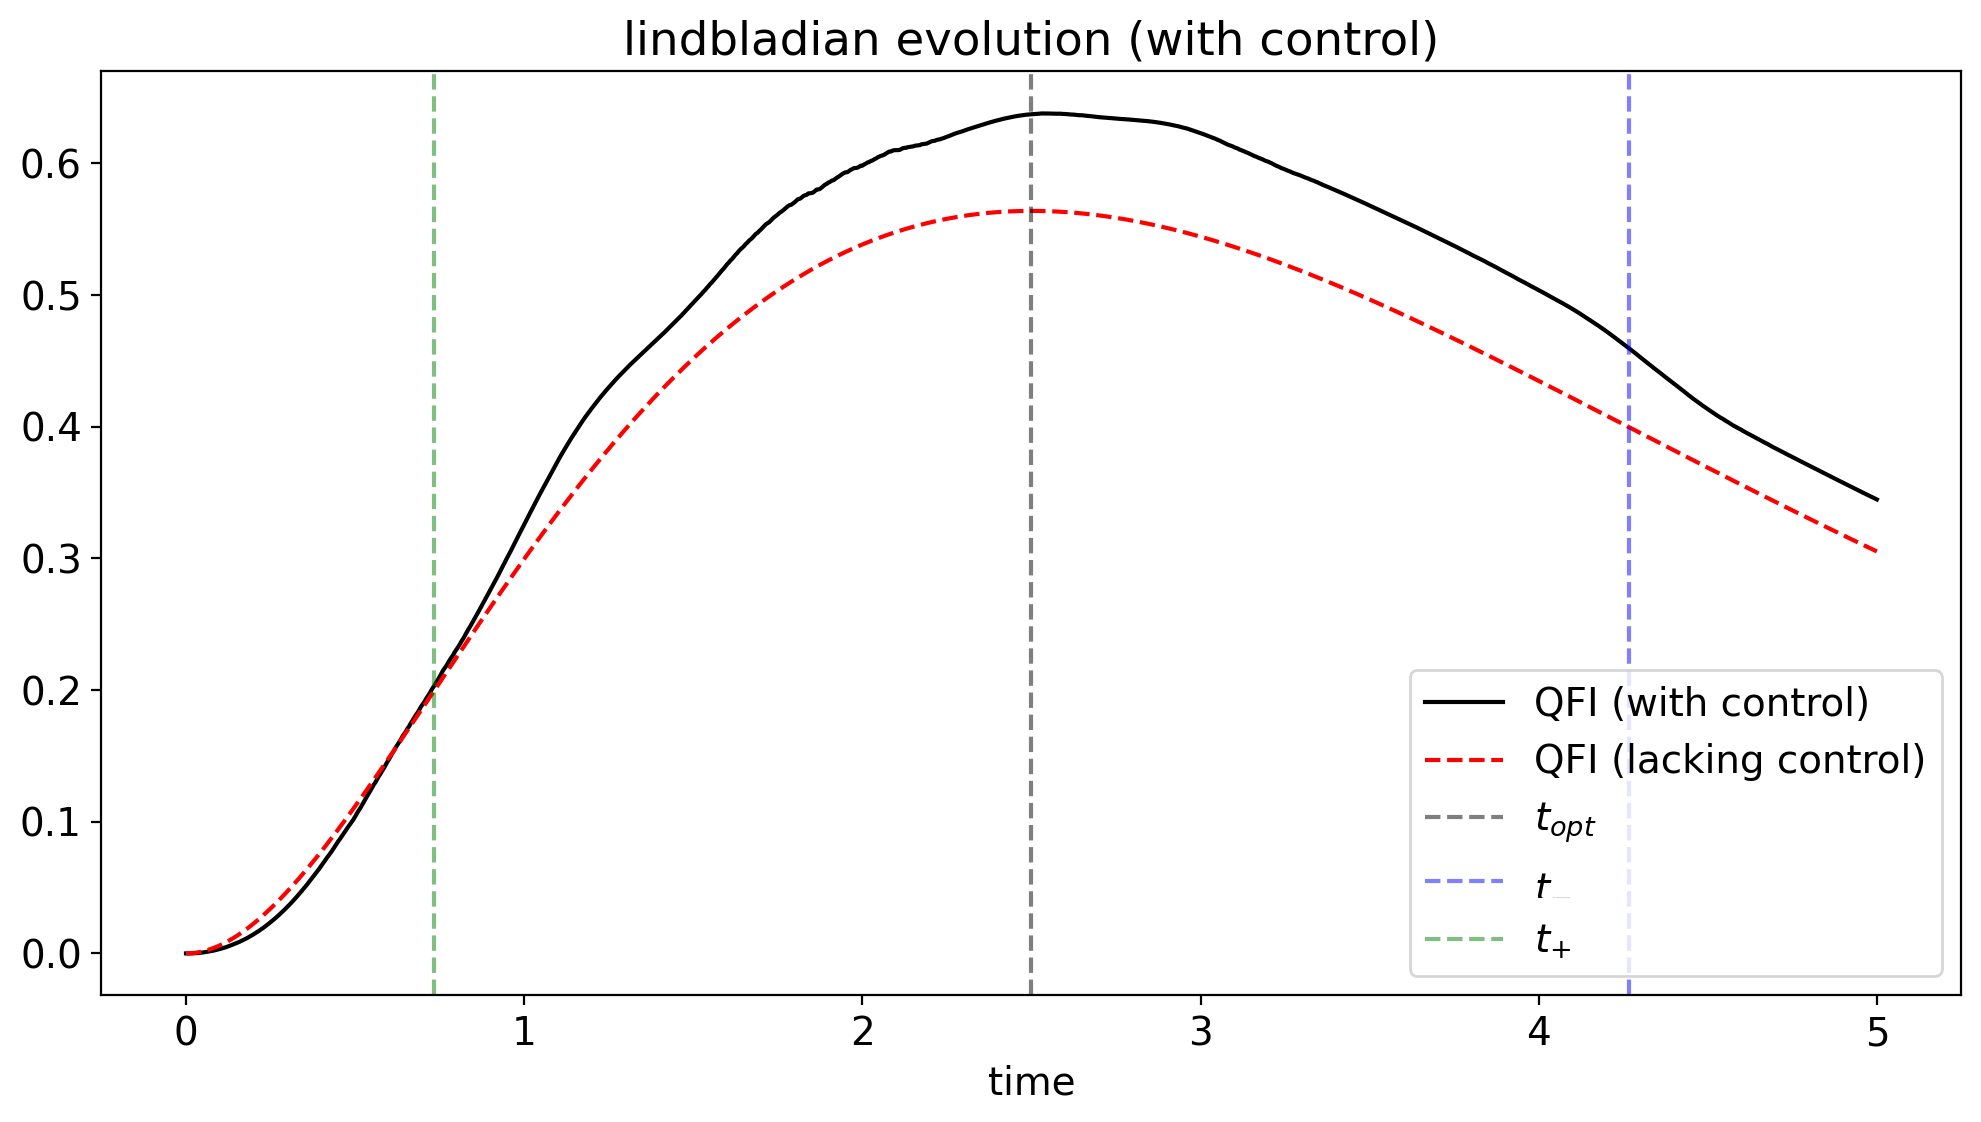
\includegraphics[width=12cm]{info_yes_control.png}
    \caption{Quantum Fisher information with respect to $\omega$.}
    \label{fig: info_yes_control}
    \centering
\end{figure}

The second control that I found is 
\begin{align}
    \vec{V}(t) = 0.5 (\cos(t), \cos(0.1 t), 1-e^{-0.1 t}).
\end{align}
Its dynamics are solved and shown in \ref{fig: bloch_yes_control2}. The quantum Fisher information improvement is shown in \ref{fig: info_yes_control2}.
\begin{figure}[ht]
    \centering
    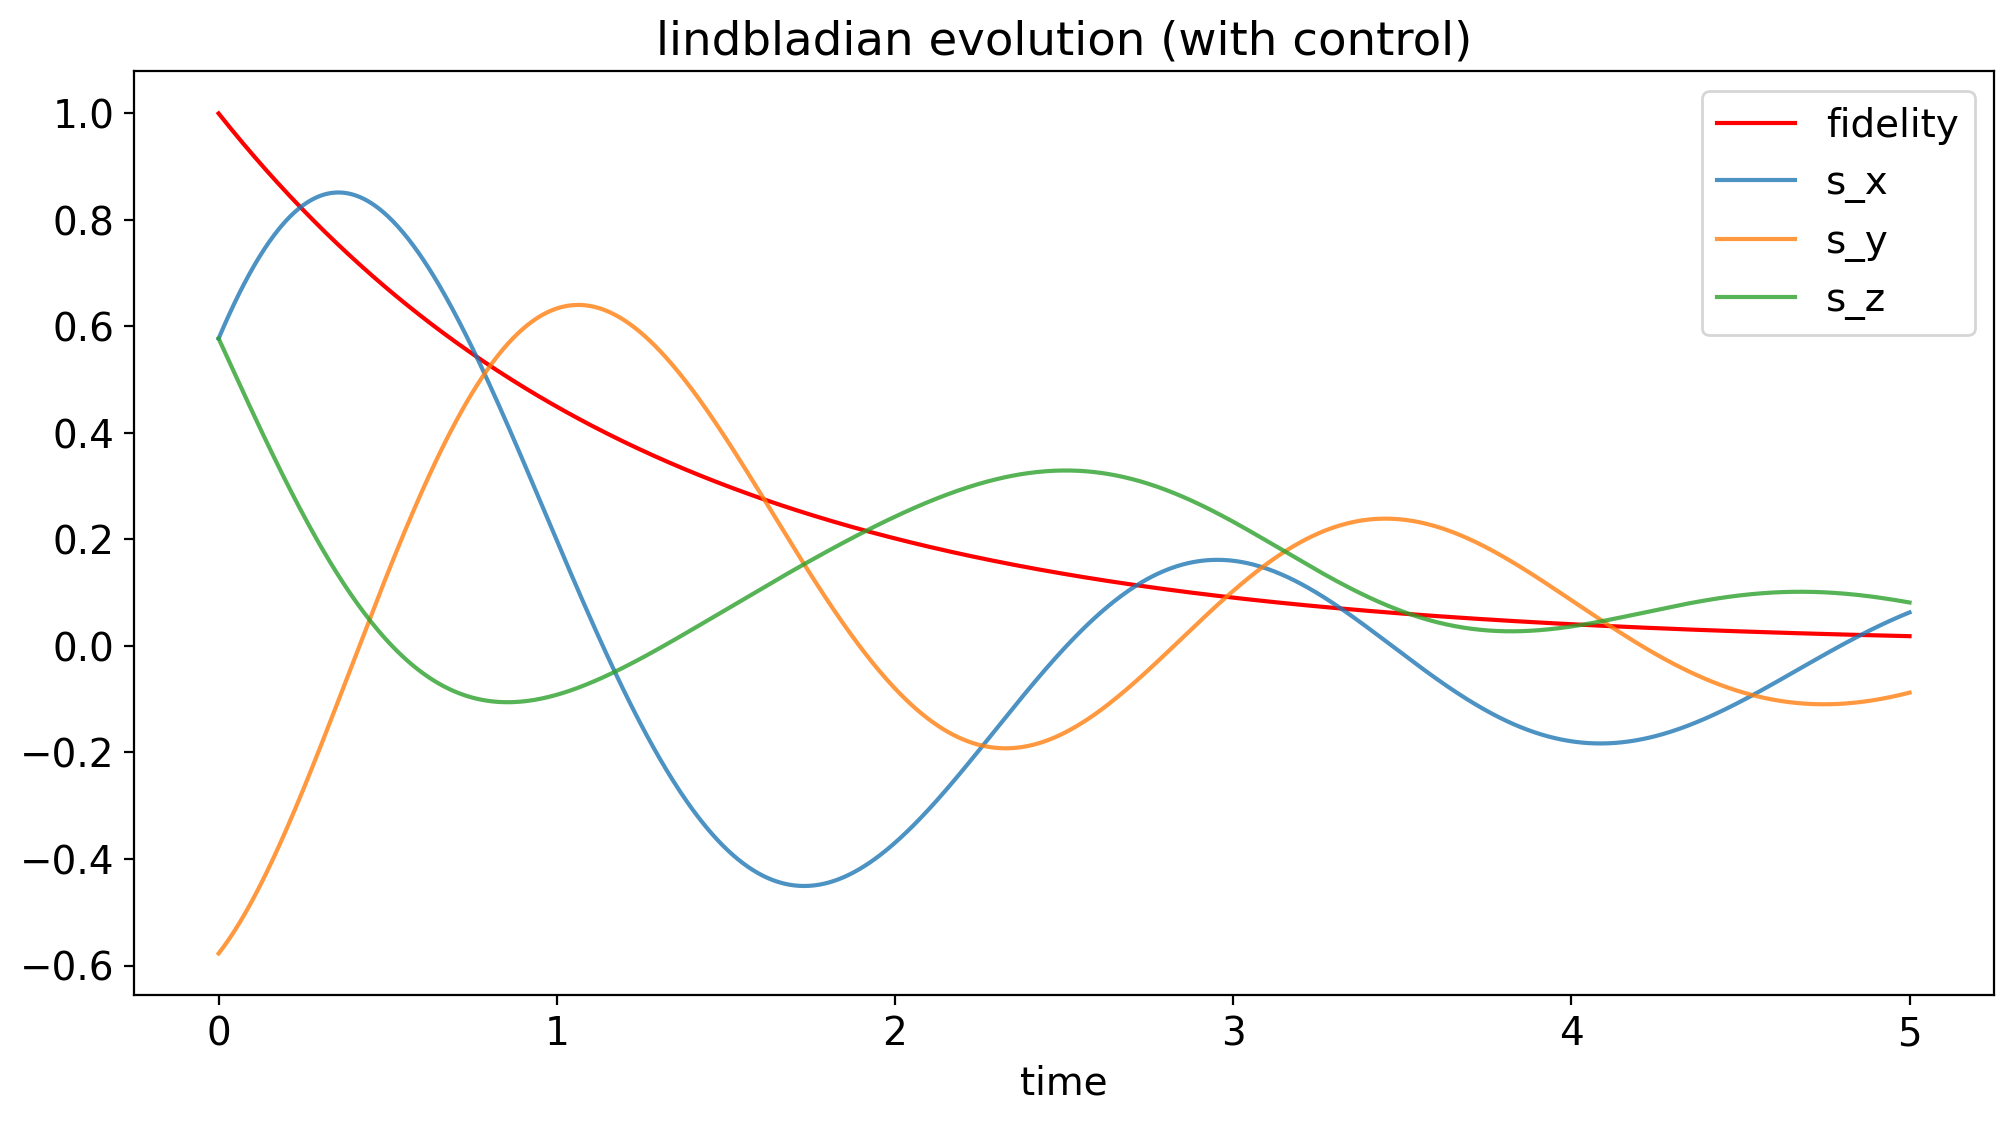
\includegraphics[width=12cm]{bloch_yes_control2.png}
    \caption{Bloch sphere dynamics and fidelity.}
    \label{fig: bloch_yes_control2}
    \centering
\end{figure}
\begin{figure}[ht]
    \centering
    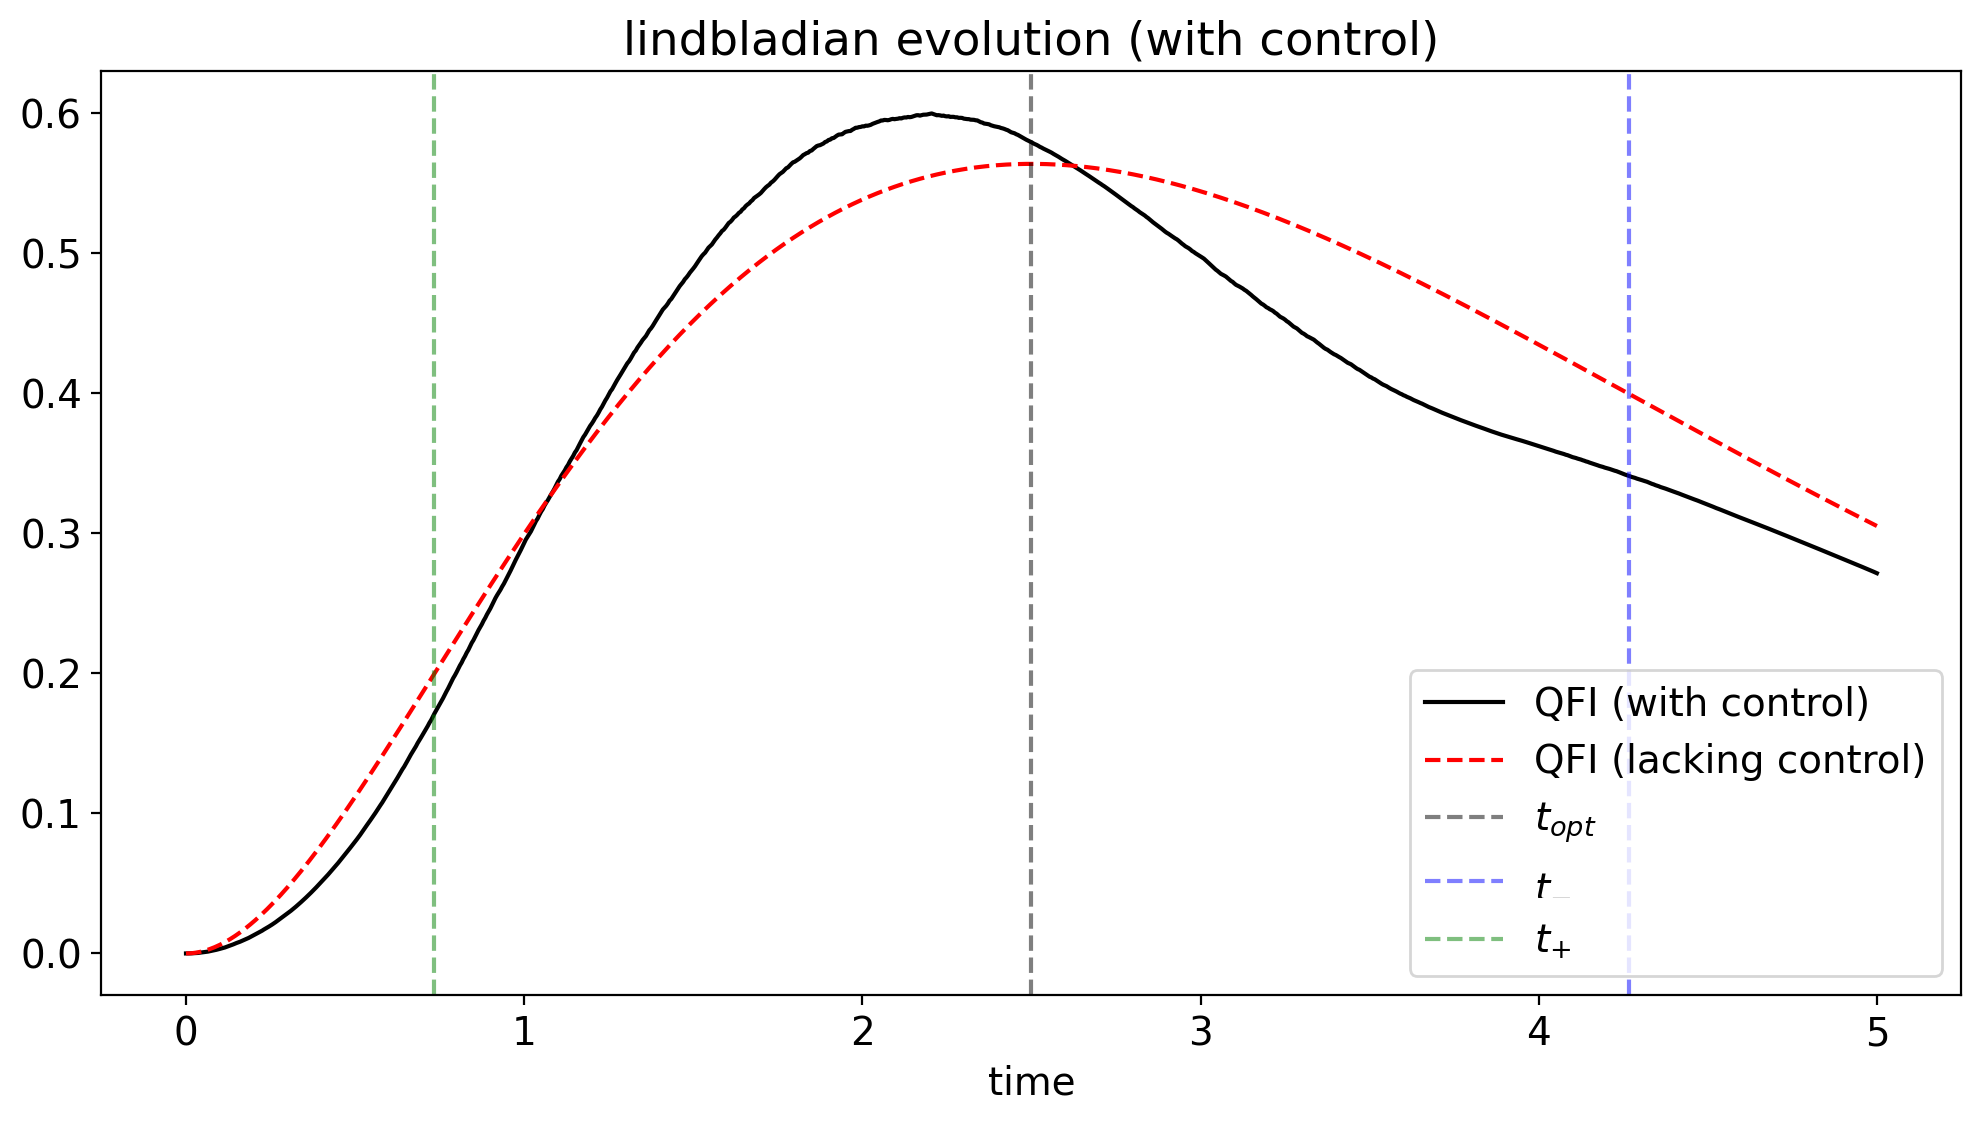
\includegraphics[width=12cm]{info_yes_control2.png}
    \caption{Quantum Fisher information with respect to $\omega$.}
    \label{fig: info_yes_control2}
    \centering
\end{figure}


My numerical results show that it is possible to choose controls that improve the quantum Fisher information in two ways: (i) $F_Q$ reaches a higher value, and (ii) $F_Q$ attains its maximum in a shorter time. For quantum sensing purposes, one should judiciously choose a control protocol $\vec{V}(t)$ to improve performance. The caveat is that the space of possible controls is too large! Brute force will fail, so one needs to resort to a more efficient method of determining the optimal control $\vec{V}(t)$. 

\newpage

\section{Reinforcement learning}

Reinforcement learning provides a platform for performing optimal control.  This note presents a scheme for sensing an external field $\vec{x}$ via controls $\vec{V}(t)$.  In an ideal setting, one tries to maximise the quantum Fisher information over infinite-time dynamics
\begin{align}
    F(\rho_0) = & \max_{\vec{V}_t} \left[ \int dt \, \gamma^t F_{Q}(\rho(t), \vec{V}(t)) \right] \\
    \text{subject to:} & \quad \partial_t \rho(t) = \mathcal{L}[\rho(t)]
\end{align}
I will make two simplifications for our purposes: (i) discretise the evolution and (ii) set a limit on the evolution.  The simplifications render the problem of finding the optimal control $\vec{V}_t$ amenable to a digital computer.  The new reward function is
\begin{align}
    F(\rho_0) = & \max_{\vec{V}_0, \cdots \vec{V}_{N-1}} \left[ \sum_{k=0}^{N-1} \, \gamma^k F_{Q}(\rho_k, \vec{V}_k) \right] \\
    \text{subject to:} & \quad \rho_{k+1} = e^{\Delta t \mathcal{L}_k} \rho_{k},
\end{align}
where $T/N = \Delta t$.

Two broad methods of determining the optimal control are off-policy and on-policy.  Q-learning is a famous off-policy method, while policy-gradient is a popular on-policy method.  I find the optimal control sequence $\vec{V}_t$ using on-policy-based methods because they are robust to errors and amenable to continuous actions.

I parameterise the policy $\pi$ in policy gradient using a flexible function approximation, such as a deep neural network.  Then, I update the parameters to optimise the reward.  For example, I want to maximise the expected reward of the policy
\begin{align}
    J(\theta) = & \E_{\pi_\theta}[F_Q]\\
    = & \int_{\mathcal{S}}d \mu(s) \, \int_{\mathcal{A}} d \nu(a) \, \pi_{\theta}(a|s)R(s,a)\\
    = & \int d \mu(\rho) \, \int d^3 \vec{V} \, \pi_{\theta}(\vec{V}|\rho)F_Q(\rho, \vec{V}).
\end{align}
\end{document}
